% !TeX spellcheck = hu_HU
% !TeX encoding = UTF-8
\chapter{Háttérismeretek}\label{sec:hatterismeretek}
\section{Esettanulmány}
Az ebben a fejezetben bemutatásra kerülő különböző adatmodellek és lekérdezőnyelvek összehasonlítása egy közös, gráf alapú adathalmazon fog történni, így először ezt mutatom be. A példa egy közösségi háló lehetséges adatbázisának egy részlete. \Aref{fig:example-graph}.~ábrán látható a példa gráfos ábrázolása, melyről leolvashatóak az alábbi adatok:
\begin{itemize}
	\item \textbf{Bob}: \uline{53 éves}, \uline{angolul} és \uline{németül} beszél.
	\item \textbf{Alice}: \uline{24 éves}, \uline{angolul} beszél, \textit{érdeklődik} a \textbf{Neofolk} iránt. \textbf{Alice} \textit{ismeri} \textbf{Bob}ot.
	\item A \textbf{Neofolk} \textit{egy} \textbf{Népzene}i műfaj.
	\item A \textbf{Népzene} \textit{része} a \textbf{Zené}nek, amely \textit{része} a \textbf{Művészet}nek.
\end{itemize}
A példa tehát \textbf{csúcsok}ból (csomópontokból), azok \uline{tulajdonság}aiból és a csúcsok között lévő kapcsolatokból, azaz \textit{élek}ből áll.
\begin{figure}[h]
	\centering
	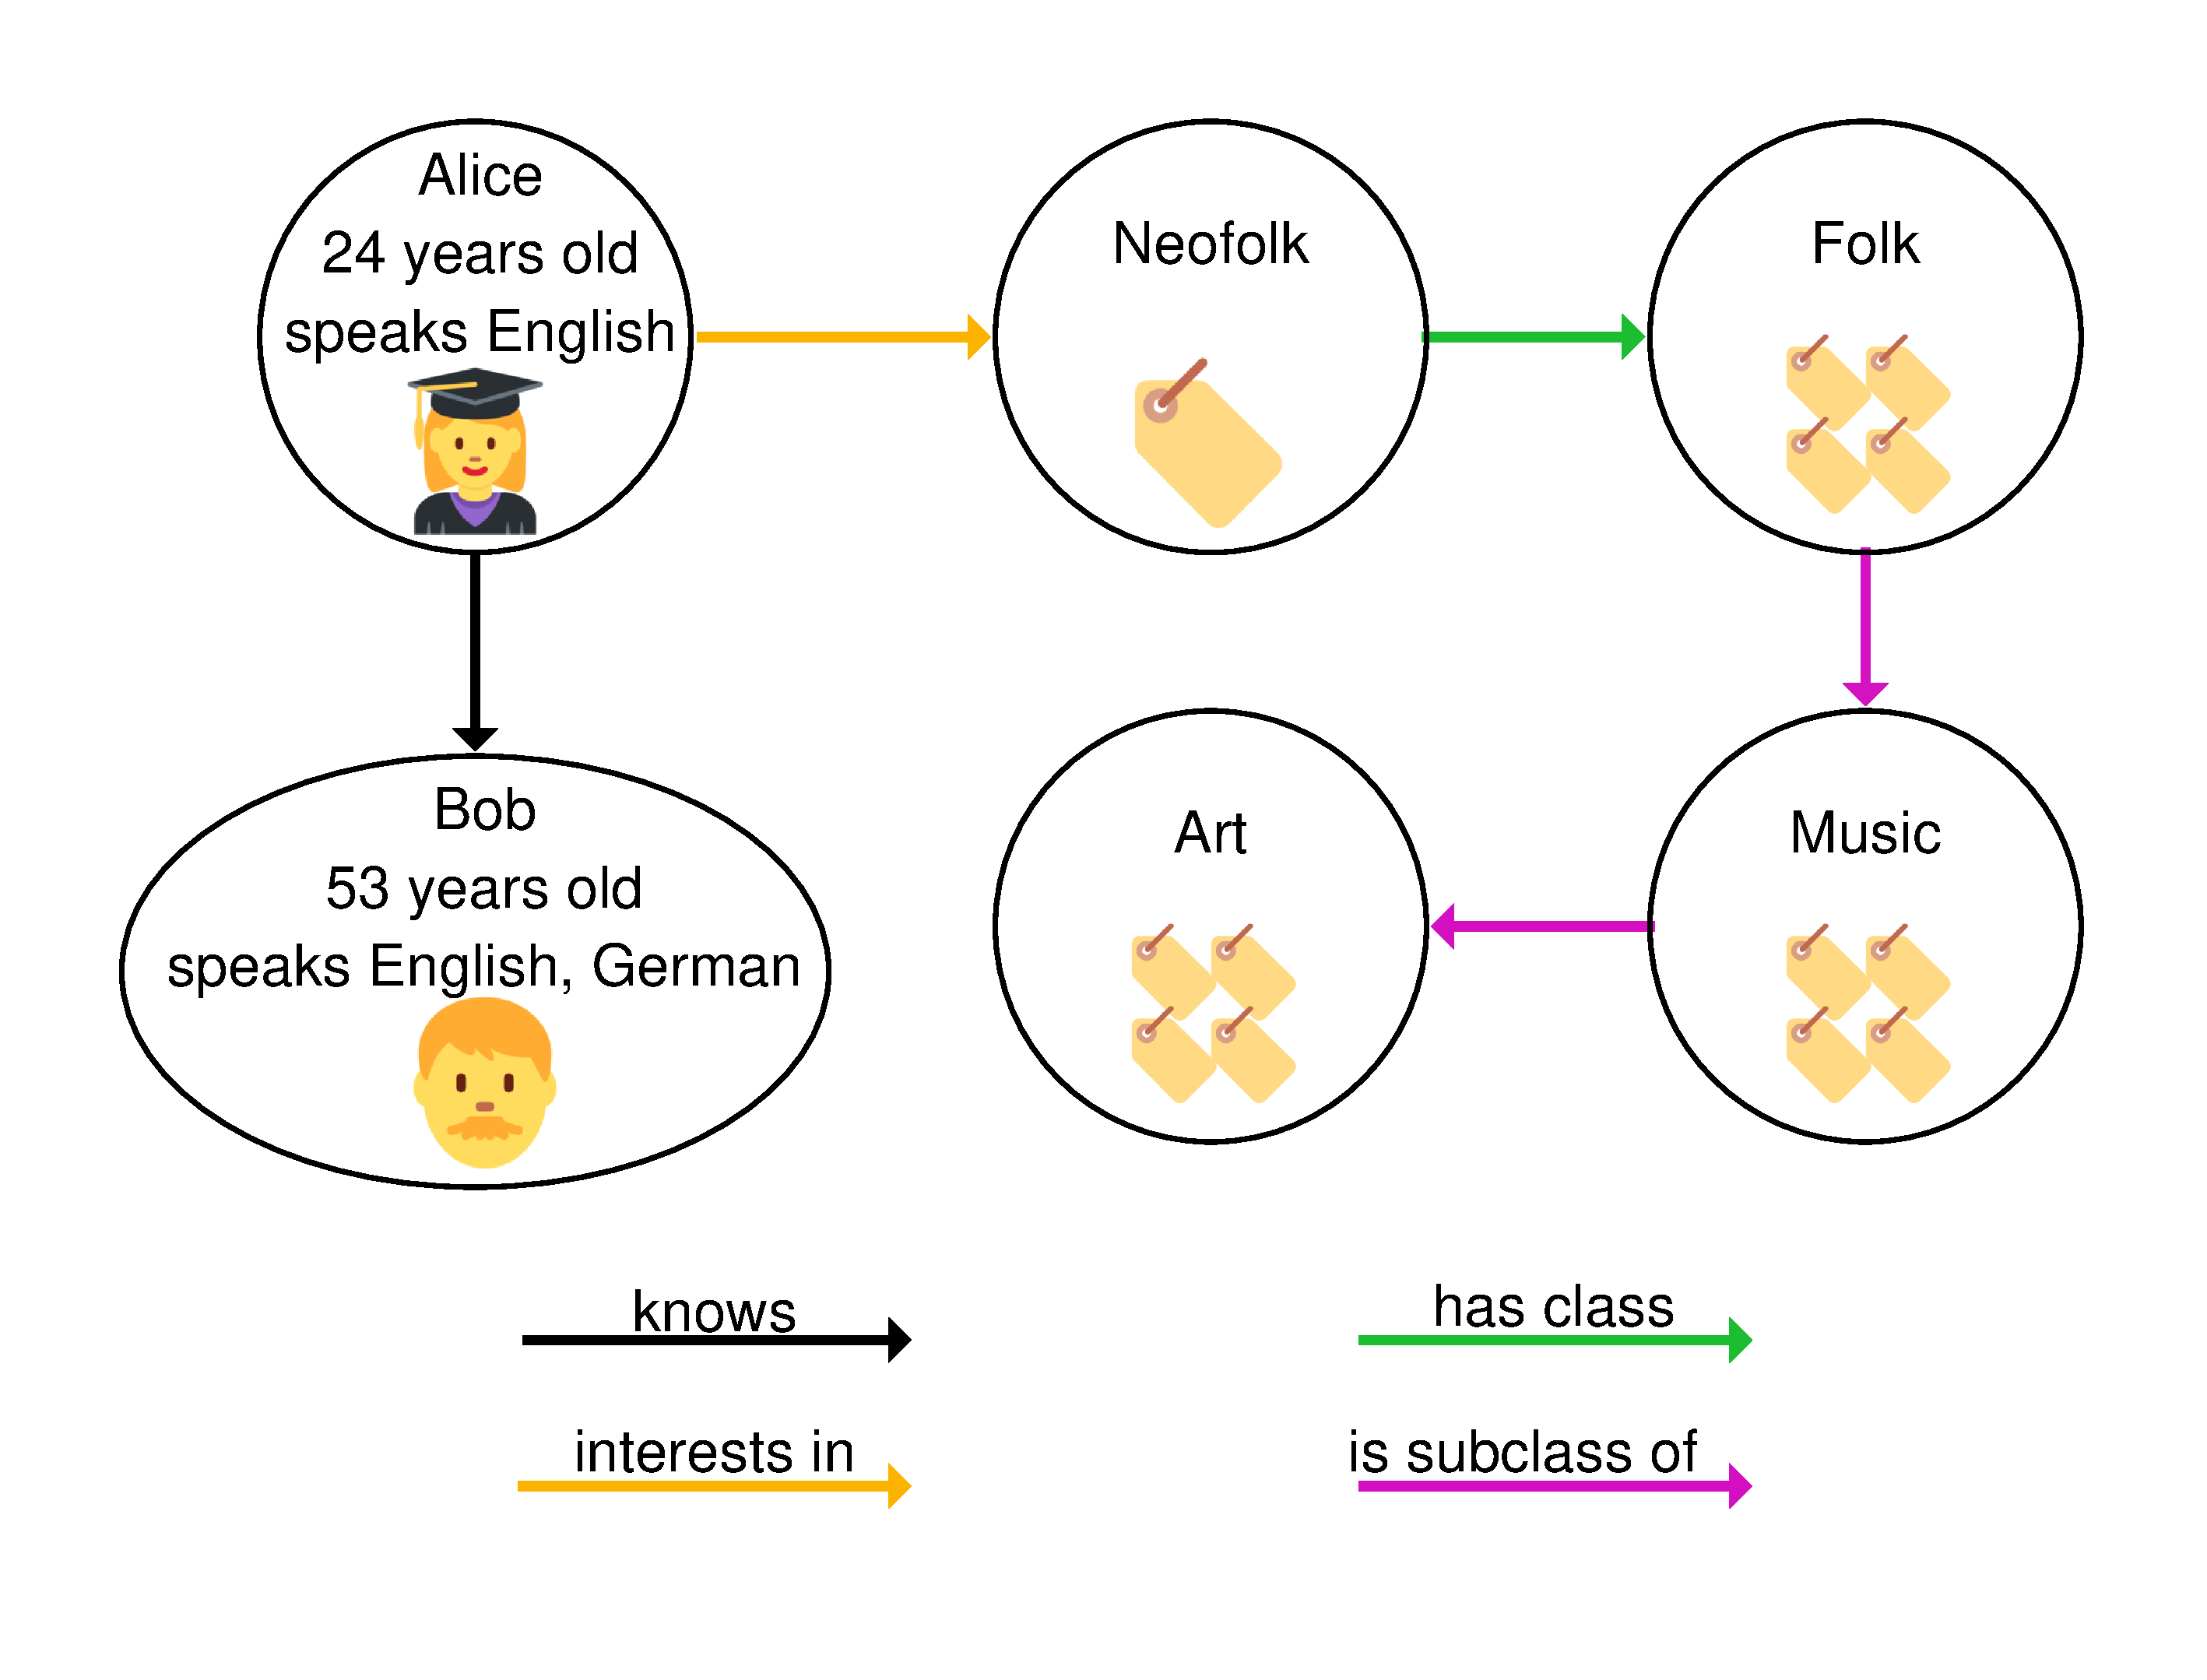
\includegraphics[scale=0.24]{example-graph.pdf}
	\caption{A példa gráf}
	\label{fig:example-graph}
\end{figure}
\section{Adatmodellek}
Az adatmodellek a példában megismert alkotórészek (csúcsok, élek és tulajdonságok) lehetséges használatának, jellemzőinek szempontjából igen különbözőek. Ezeket a különbségeket mutatja be \aref{tab:datamodels}.~táblázat. Jól látható, hogy a spektrum egyik vége a matematikában is megszokott irányított gráfok, a másik vége pedig az egyik legújabb adatmodell, a tulajdonsággráf. Az irányított gráfokkal ellentétben a címkézett gráfok csúcsainak már lehetnek típusai, amelyeket a megfelelő címkék csúcshoz rendelésével lehet meghatározni. Ha egy gráf csúcsain kívül az éleit is címkékkel látjuk el, akkor szemantikus gráfot kapunk. A tulajdonsággráf esetében a gráf csúcsainak és éleinek nem csak típusuk, hanem tulajdonságaik is lehetnek. Egy tulajdonság az egyszerű numerikus vagy szöveges adattípusokon túl akár komplexebb típus is lehet, például lista vagy halmaz.

A táblázatban továbbá látható az objektum-orientált modell, amely nem egyértelmű, hogyan kapcsolódik a gráf alapú adatmodellekhez: ha egy címkézett gráf csúcsainak lehetnek tulajdonságai, akkor az megfeleltethető a széles körben használt objektum-orientált modellnek. Fontos megjegyezni, hogy elméletben az objektum-orientált modellben is lehet az éleknek tulajdonsága, de ezt a gyakorlati megvalósítások közül elhanyagolható számú támogatja csupán. A továbbiakban három adatmodell kerül részletes bemutatásra a táblázatból: a szemantikus gráfok, a tulajdonsággráfok és a relációs adatmodell.
\begin{table}[h]
	\centering
	\begin{tabular}{@{\extracolsep{4pt}}lcccc@{}}
		\toprule
		\multicolumn{1}{c}{\multirow{3}{*}{adatmodell}} & \multicolumn{4}{c}{adatmodell tulajdonság} \\
		\cline{2-5}
		 & \multicolumn{2}{c}{csúcsok} & \multicolumn{2}{c}{élek} \\
		 \cline{2-3} \cline{4-5}
		 & típus & tulajdonság & típus & tulajdonság \\
		\midrule
		irányított gráf & $\circ$ & $\circ$ & $\circ$ & $\circ$ \\
		címkézett gráf & $\bullet$ & $\circ$ & $\circ$ & $\circ$ \\
		szemantikus gráf & $\bullet$ & $*$ & $\bullet$ & $\circ$ \\
		objektum-orientált modell & $\bullet$ & $\bullet$ & $\bullet$ & $\circ$ \\
		tulajdonsággráf & $\bullet$ & $\bullet$ & $\bullet$ & $\bullet$ \\
		\bottomrule
	\end{tabular}
	\caption{Az adatmodellek tulajdonságainak összehasonlítása}
	\label{tab:datamodels}
\end{table}
\subsection{Tulajdonsággráf}
A \emph{tulajdonsággráf} (property graph, PG) egy $G = (V, E, \verticestoedges, \vertexlabels, \edgelabels, \vertexlabelfunction, \edgelabelfunction, \vertexproperties, \edgeproperties)$ struktúrával írható le, ahol $V$ a csúcsok (csomópontok) halmaza, $E$ az élek halmaza és $\verticestoedges: E \assign V \cartesianproductop V$ függvény határozza meg az élek kiindulási és cél csúcsát~\cite{DBLP:conf/adbis/MartonSV17}. Formálisan a csúcsok típusát címkének nevezzük, az élek esetében pedig formálisan is típusról beszélünk:
\begin{itemize}
	\item $\vertexlabels$ a címkék halmaza, a $\vertexlabelfunction: V \assign 2^{\vertexlabels}$ függvény pedig \emph{a címkék egy halmazát} rendeli a csúcsokhoz.
	\item $\edgelabels$ a típusok halmaza, a $\edgelabelfunction: E \assign \edgelabels$ függvény pedig \emph{pontosan egy típust} rendel minden élhez.
\end{itemize}

A tulajdonságok definiálásához legyen $D = \bigcup_i D_i$ a különböző $D_i$ elemi domének uniója, és legyen $\relnull$ a \texttt{NULL} érték.
\begin{itemize}
	\item $\vertexproperties$ a csúcsok tulajdonságainak halmaza. A $p_i \in \vertexproperties$ csúcstulajdonság egy függvény $p_i: V \assign D_i \unionop \{ \relnull \}$, amely egy csúcstulajdonság értéket rendel a $D_i \in D$ doménből a $v \in V$ csúcshoz, ha $v$ rendelkezik a $p_i$ csúcstulajdonsággal, egyébként $p_i(v)$ értéke $\relnull$.
	\item $\edgeproperties$ az élek tulajdonságainak halmaza.A $p_j \in \edgeproperties$ éltulajdonság egy függvény $p_j: E \assign D_j \unionop \{ \relnull \}$, amely egy éltulajdonságot rendel a $D_j \in D$ doménből az $e \in E$ élhez, ha $e$ rendelkezik a $p_j$ éltulajdonsággal, egyébként $p_j(e)$ értéke $\relnull$.
\end{itemize}
A továbbiakban a csúcs- és éltulajdonságokat is tulajdonságnak hívjuk, csak ott különböztetjük meg őket ahol a megértés könnyebbsége miatt szükséges. 

Legyen $r$ reláció n-esek egy \emph{multihalmaza} (bag). Ekkor $r$ egy gráf reláció a $G$ tulajdonsággráfon, ha igaz az alábbi:

$$\forall A \in \schema{r}: \dom{A} \subseteq V \union E \union D,$$

ahol $sch(r)$ jelöli $r$ sémáját, azaz $r$-ben lévő attribútumok neveinek listáját, $dom(A)$ az $A$ attribútum doménjét, továbbá $V$ és $E$ a definíció szerint a gráf csúcsait és éleit jelölik. 

\Aref{fig:example-pg}.~ábrán látható a példa gráf tulajdonsággráf vizuális modellje, a tulajdonsággráf formális modellje pedig az alábbi:

\begin{align*}
	\vertexlabels &= \{\atom{Person}, \atom{Student}, \atom{Class}, \ldots \}\\
	\edgelabels &= \{\atom{KNOWS}, \atom{INTEREST}, \atom{CLASS}, \atom{SUBCLASS\_OF}\}\\
	\vertexproperties &= \{\atom{name}, \atom{speaks}, \atom{age}, \ldots\}\\
	\edgeproperties &= \{\atom{since}\}\\
	V &= \{a, b, c, d, e, f\}\\E &= \{1, 2, 3, 4, 5\}\\
	\verticestoedges&:\ 1 \assign \tuple{a, c}, 2 \assign \tuple{b, c}, \ldots\\
	\vertexlabelfunction&:\ b \assign \{\atom{Person}\}, a \assign \{\atom{Person}, \atom{Student}\}, \ldots\\
	\edgelabelfunction&:\ 1 \assign \atom{KNOWS}, 3 \assign \atom{CLASS}, \ldots\\
	\atom{name}&:\ a \assign \atom{``Alice"}, b \assign \atom{``Bob"}, e \assign \relnull, \ldots\\
	\atom{since}&:\ 1 \assign \atom{2014}, 2 \assign \relnull, 3 \assign \relnull, \ldots \\
	\ldots
%	\atom{age}&:\ \ldots\\
%	\atom{speaks}&:\ \ldots\\
%	\atom{topic}&:\ \ldots\\
%	\atom{level}&:\ \ldots\\
%	\atom{subject}&:\ \ldots
\end{align*}
\begin{figure}
	\centering
	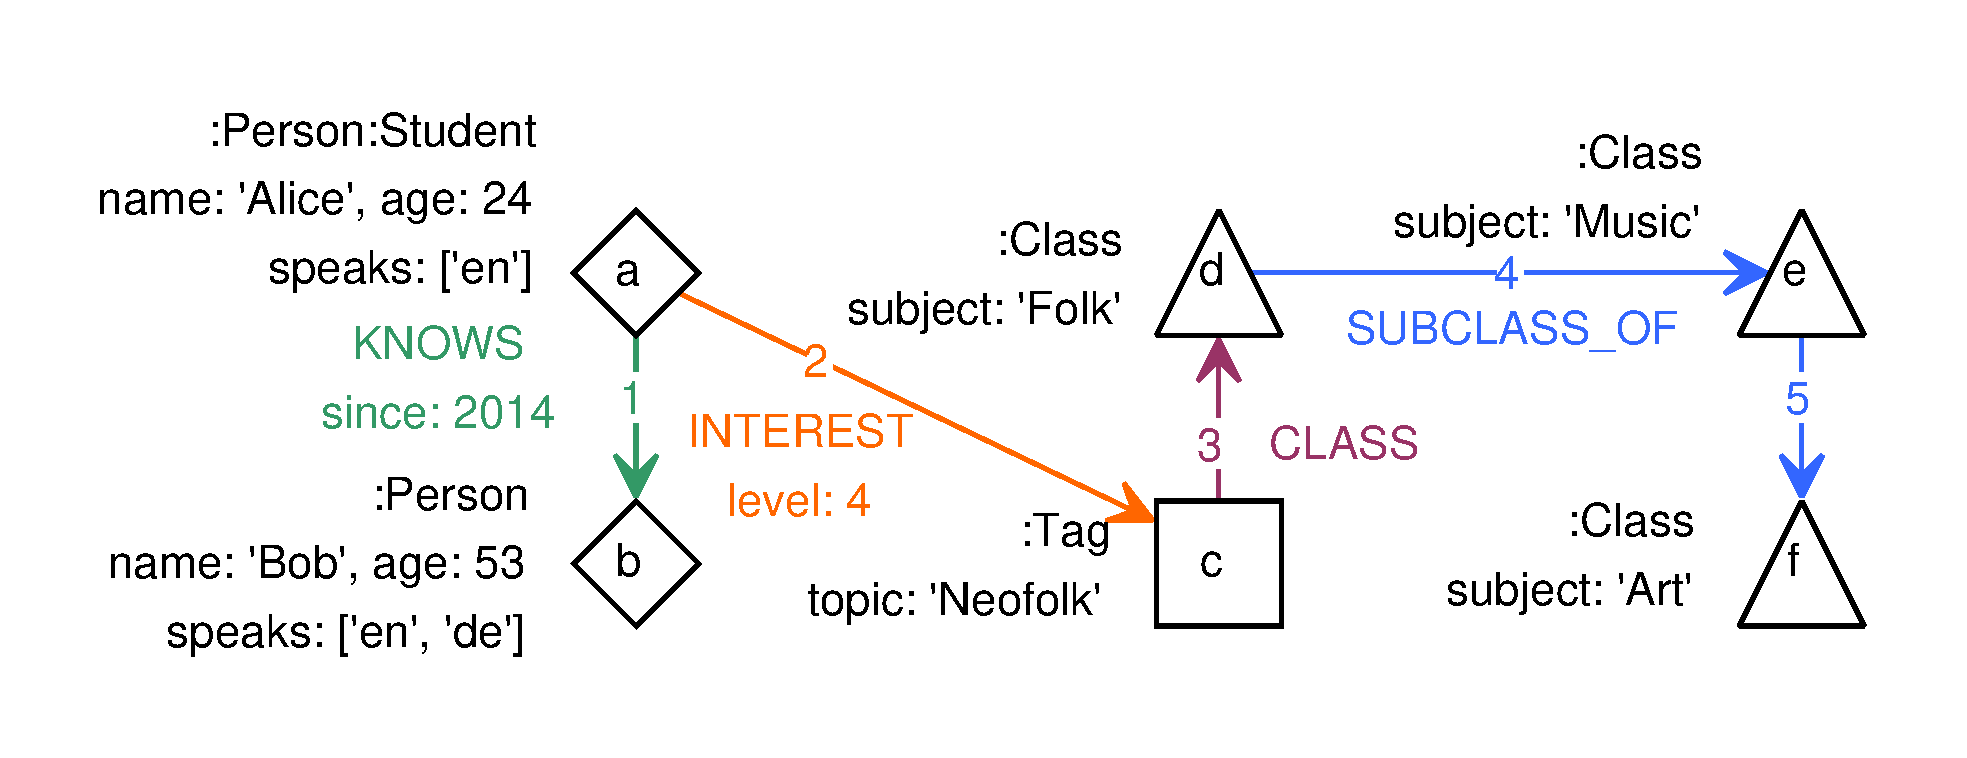
\includegraphics[scale=0.32]{example-pg.pdf}
	\caption{A példa tulajdonsággráf modellje. $\Diamond$~Person, $\Box$~Tag, $\triangle$~TagClass}
	\label{fig:example-pg}
\end{figure}
\subsection{Szemantikus gráf}

A szemantikus gráf olyan speciális adatmodell, amelyben egy gráfban találhatóak a metamodell és a példánymodell elemei. A szemantikus gráfnak számos reprezentációja létezik, ezek közül az egyik leggyakoribb a World Wide Web Consortium (W3C)\footnote{\url{https://www.w3.org/}} gondozásában lévő Resource Description Framework (RDF)\footnote{\url{https://www.w3.org/standards/techs/rdf}}. Mivel az RDF pontos definíciója meghaladja e dolgozat kereteit, ezért csak a legfontosabb részeket emeltem ki a specifikációból.

Egy RDF gráf hármasok egy halmaza. Egy hármas elemei az alábbiak:
\begin{itemize}
	\item alany, amely egy IRI hivatkozás vagy egy üres csomópont
	\item állítmány, amely egy IRI hivatkozás
	\item tárgy, amely egy IRI hivatkozás, egy literál vagy üres csomópont
\end{itemize}
Az IRI\footnote{Formális definíció:\url{ https://www.w3.org/TR/2014/REC-rdf11-concepts-20140225/\#section-IRIs}} (Internationalized Resource Identifier) egy UNICODE karakterlánc, amely egyértelműen azonosítja a gráf elemeit. Egy RDF gráfban az üres csomópontokat egy végtelen halmazból nyerjük. Az üres csomópontoknak ez a halmaza, továbbá az összes IRI hivatkozás halmaza, valamint az összes literál halmaza páronként diszjunkt halmazokat alkotnak. Formálisan tehát legyen $I$ az IRI-k halmaza, $B$ az üres csomópontok halmaza, $L$ pedig a literálok halmaza, akkor az $(s,p,o) \in (I \union B) \times I \times (I \union B \union L)$ egy RDF hármas, ahol $s$ az alany, $p$ az állítmány és $o$ a tárgy. A példa egy részletének megfelelő RDF szöveges reprezentációja\footnote{N-Triples formátumról bővebben: \url{https://www.w3.org/TR/n-triples/}}:
\begin{lstlisting}[frame=single]
a type Person .
a type Student .
a name "Alice" .
a age 24 .
a knows _:tmp1 .
_:tmp1 hasPerson b .
b name "Bob" .
\end{lstlisting}
Ebben példában az IRI-k halmaza $\{a, b, Person, Student, type, name, age, knows, hasPerson\}$, a literálok halmaza $\{``Alice", ``Bob", 24\}$ és az üres csomópontok halmaza pedig $\{_:tmp1\}$.

\begin{figure}[h]
	\centering
	\includegraphics[scale=0.2]{triple.pdf}
	\caption{Egy RDF hármas grafikus ábrázolása}
	\label{fig:triple}
\end{figure}

\begin{figure}
\centering
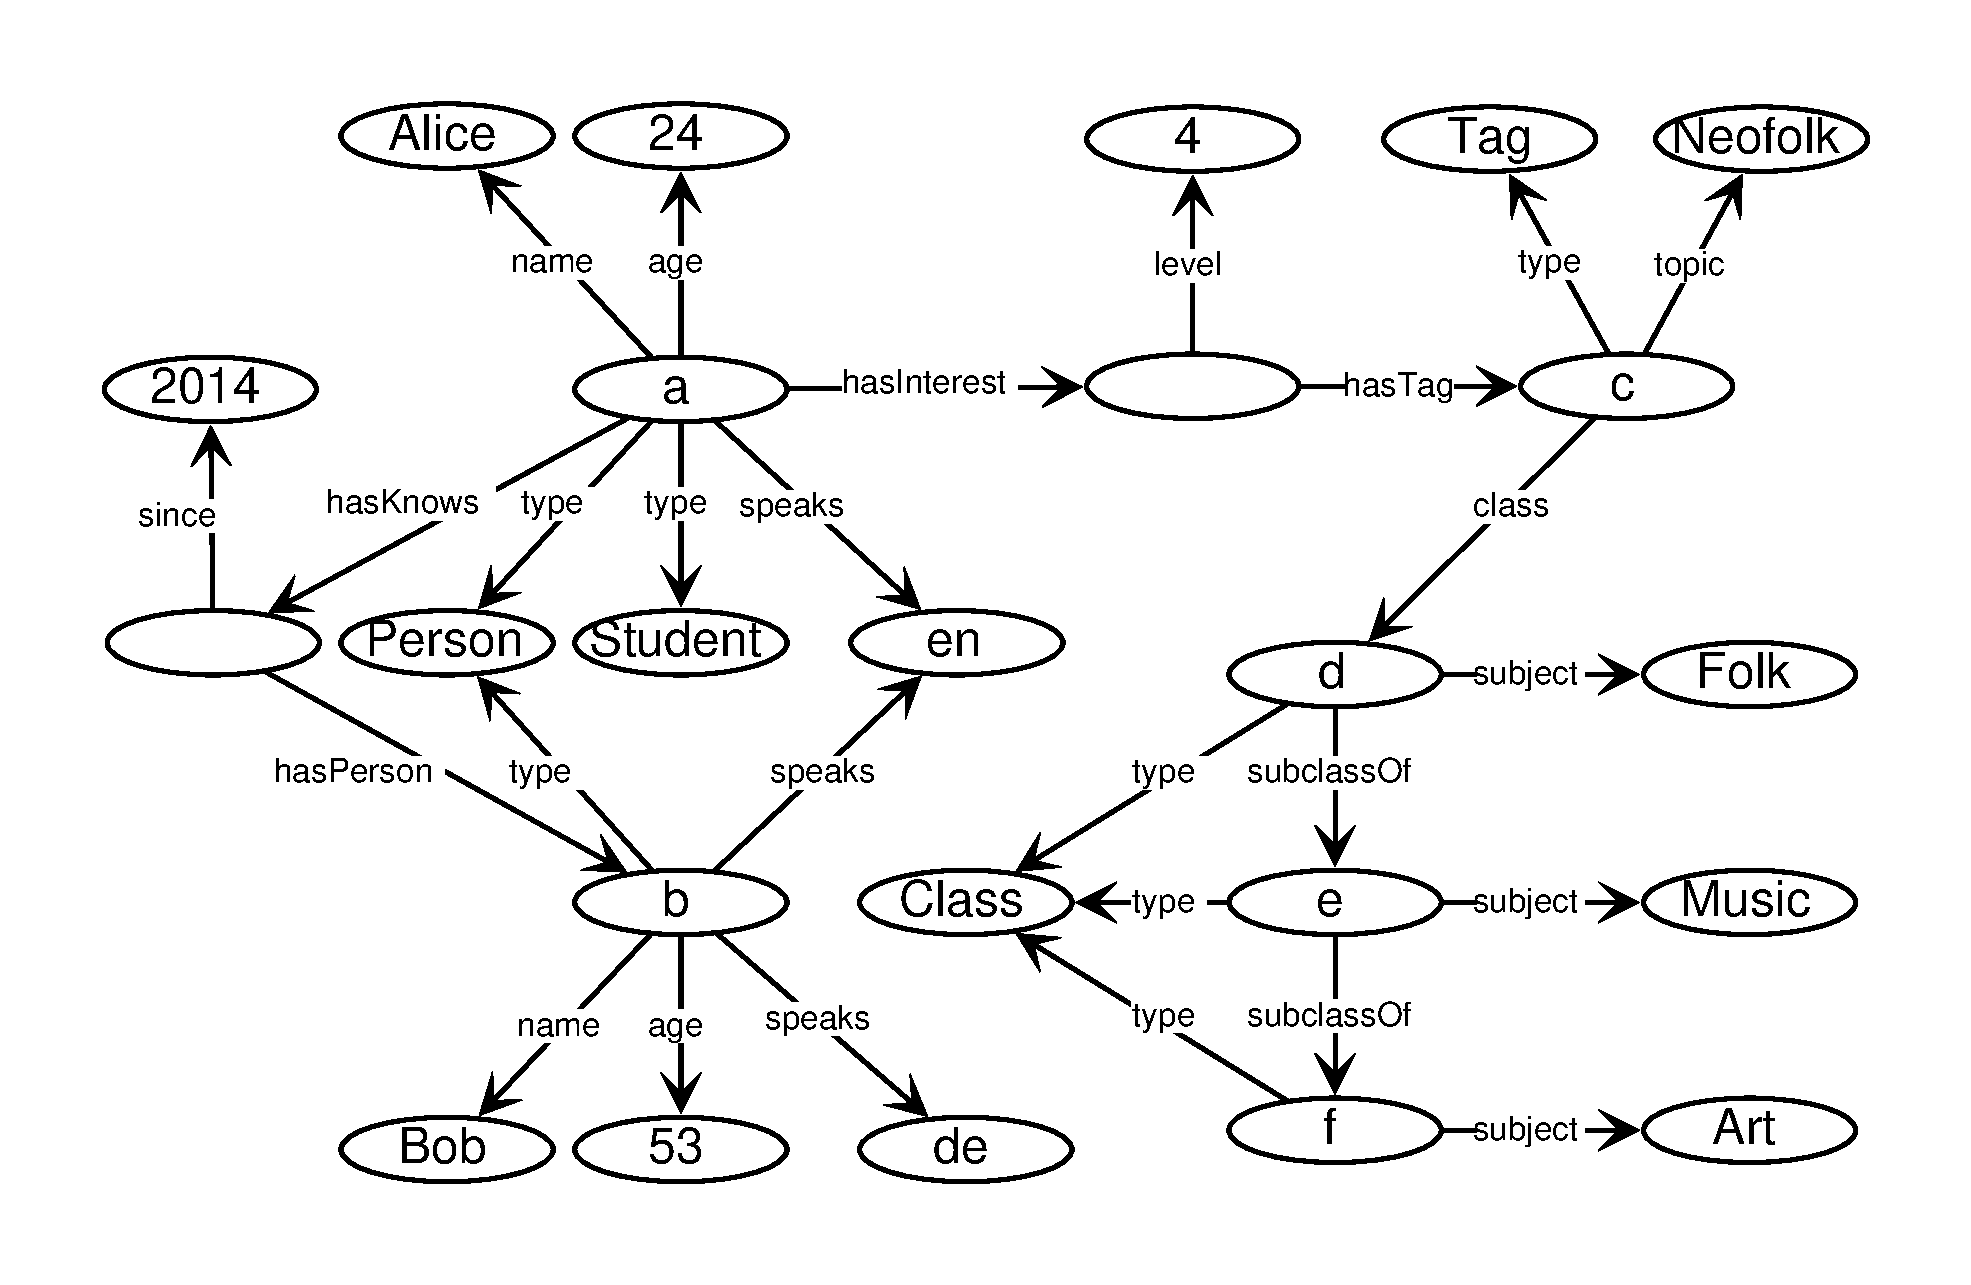
\includegraphics[scale=0.45]{example-rdf.pdf}
\caption{A példa RDF gráf modellje}
\label{fig:example-rdf}
\end{figure}

Az RDF gráf csomópontjainak halmazát a gráf hármasainak alanyai és tárgyai alkotják, az élek halmazát pedig a gráf hármasainak állítmányai alkotják. Egy hármas grafikusan ábrázolható két csomóponttal és a közöttük lévő irányított éllel, ahogy \aref{fig:triple}.~ábrán látható. Ilyen módon megkaphatjuk a példa RDF gráf modelljének \aref{fig:example-rdf}.~ábrán látható grafikus vizualizációját. Az ábrán látható, hogy az RDF gráfok csúcs- és élcímkézett irányított gráfok.

\Aref{tab:datamodels} táblázat szemantikus gráfhoz tartozó sorában látható $*$ azt jelenti, hogy bár egy RDF gráfban a csúcsoknak nem lehet tulajdonsága, de a csúcsok tulajdonságait egyszerűen leképezhetjük hármasokká, ahogy a példa gráf RDF gráfján látszik: az eredeti gráf \textit{name} tulajdonságát az RDF gráfban az azonos nevű állítmánnyal rendelkező hármas jelenti.

\subsection{Relációs adatmodell}
\label{sec:relacios-adatmodell}

A dolgozatban megemlített adatmodellek közül a relációs adatmodell a legrégebb óta használt és kutatott modell. Ebben a fejezetben az E. F. Codd által leírt definíciót~\cite{DBLP:journals/cacm/Codd70} ismertetem.
Adottak \set{1}, \set{2}, \dots, \set{n} nem feltétlenül különböző halmazok, ekkor \rel{} egy reláció ezen az $n$ halmazon, ha \rel{} $\subseteq{}$ \set{1} $\times$ \set{2} $\times$ \dots $\times$ \set{n}. Ilyenkor az \set{i} halmaz az \rel{} $i.$ doménje.

Gyakran a relációkat táblázatokként ábrázoljuk. Az \rel{} relációt ábrázoló táblázat minden sora megfeleltethető pontosan egy elemnek \rel{}-ből, így a reláció elemeit a reláció sorainak is nevezzük.
Az oszlopok sorrendje követi az \set{1}, \set{2}, \dots, \set{n} sorrendet, azaz az $i.$ oszlop az $i.$ domén értékeit tartalmazza. Az oszlopokat szokás a hozzájuk tartozó domén nevével felcímkézni, ezzel egyértelműsíteni a jelentésüket. Esetenként az oszlopokra egyszerűen a nevükkel hivatkozunk és nem vesszük figyelembe az attribútumok sorrendjét.

A relációk lehetnek \emph{halmaz} (set) szemantikájúak, ebben az esetben az elemeik egyediek, valamint \emph{multihalmaz} szemantikájúak, amikor az elemeiek között előfordulhatnak ismétlődések. A reláció elemeinek sorrendje egyik esetben sem számít.

A példa relációs modellje \aref{fig:example-rdf}.~ábrán látható. Megfigyelhető, hogy a példában minden csúcstípushoz (\textsf{Persons}, \textsf{Tags}, \textsf{TagClasses} relációk), minden többes kardinalitású csúcs tulajdonságához (\textsf{Speaks}) és minden éltípushoz (\textsf{Interests}, \textsf{SubclassOf}, \textsf{HasClass}) külön reláció tartozik: ez gyakori leképzése a gráfoknak a relációs adatmodellre. További fontos megfigyelés, hogy az éleket jelentő relációknak (\textsf{Knows}, \textsf{Interests}, \textsf{SubclassOf}, \textsf{HasClass}) nincsen azonosítója, mert ezeket az él kezdő- és végpontja azonosítja. Ez a séma feltételezi, hogy két csúcs között nem vezet egynél több azonos él (ugyanolyan típusú él vezethet, ha legalább egy éltulajdonságban eltérnek), továbbá hogy tanulók csak személyek lehetnek (\textsf{Students} reláció).

\begin{figure}[htb]
	\begin{subfigure}[b]{0.22\textwidth}
		\begin{center}
			\begin{tabular}{|c|l|c|}
				%\hline
				%\multicolumn{3}{|c|}{\bf persons} \\
				\hline
				id & \multicolumn{1}{|c|}{name} & age \\
				\hline
				a & Alice & 24 \\
				\hline
				b & Bob & 53 \\
				\hline \\
			\end{tabular}
			\caption{\textsf{Persons}}
			\label{example-rdb-persons}
		\end{center}
	\end{subfigure}
	\begin{subfigure}[b]{0.16\textwidth}
	\begin{center}
		\begin{tabular}{|c|c|c|}
			%\hline
			%\multicolumn{3}{|c|}{\bf interests} \\
			\hline
			personId \\
			\hline
			a \\
			\hline \\ \\
		\end{tabular}
		\caption{\textsf{Students}}
		\label{example-rdb-students}
	\end{center}
	\end{subfigure}
	\begin{subfigure}[b]{0.2\textwidth}
		\begin{center}
			\begin{tabular}{|c|l|}
				%\hline
				%\multicolumn{2}{|c|}{\bf tags} \\
				\hline
				id & \multicolumn{1}{|c|}{topic} \\
				\hline
				c & Neofolk \\
				\hline \\ \\
			\end{tabular}
			\caption{\textsf{Tags}}
			\label{example-rdb-tags}
		\end{center}
	\end{subfigure}
	\begin{subfigure}[b]{0.2\textwidth}
		\begin{center}
			\begin{tabular}{|c|l|}
				%\hline
				%\multicolumn{2}{|c|}{\bf tagClasses} \\
				\hline
				id & \multicolumn{1}{|c|}{subject} \\
				\hline
				d & Folk \\
				\hline
				e & Music \\
				\hline
				f & Art \\
				\hline
			\end{tabular}
			\caption{\textsf{TagClasses}}
			\label{example-rdb-tagclasses}
		\end{center}
	\end{subfigure}
	\begin{subfigure}[b]{0.16\textwidth}
		\begin{center}
			\begin{tabular}{|c|c|}
				%\hline
				%\multicolumn{2}{|c|}{\bf hasClass} \\
				\hline
				tag & class\\
				\hline
				c & d \\
				\hline \\ \\
			\end{tabular}
			\caption{\textsf{HasClass}}
			\label{example-rdb-hasClass}
		\end{center}
	\end{subfigure}

	\

	\begin{subfigure}[b]{0.2\textwidth}
		\begin{center}
			\begin{tabular}{|c|c|}
				%\hline
				%\multicolumn{2}{|c|}{\bf subclassOf} \\
				\hline
				src & trg\\
				\hline
				d & e \\
				\hline
				e & f \\
				\hline \\
			\end{tabular}
			\caption{\textsf{SubclassOf}}
			\label{example-rdb-subclassOf}
		\end{center}
	\end{subfigure}
	\begin{subfigure}[b]{0.26\textwidth}
		\begin{center}
			\begin{tabular}{|c|c|c|}
				%\hline
				%\multicolumn{3}{|c|}{\bf knows} \\
				\hline
				src & trg & since\\
				\hline
				a & b & 2014 \\
				\hline \\ \\
			\end{tabular}
			\caption{\textsf{Knows}}
			\label{example-rdb-knows}
		\end{center}
	\end{subfigure}
	\begin{subfigure}[b]{0.28\textwidth}
		\begin{center}
			\begin{tabular}{|c|c|c|}
				%\hline
				%\multicolumn{3}{|c|}{\bf interests} \\
				\hline
				person & tag & level\\
				\hline
				a & d & 4 \\
				\hline \\ \\
			\end{tabular}
			\caption{\textsf{Interests}}
			\label{example-rdb-interests}
		\end{center}
	\end{subfigure}
	\begin{subfigure}[b]{0.24\textwidth}
	\begin{center}
		\begin{tabular}{|c|c|}
			%\hline
			%\multicolumn{2}{|c|}{\bf speaks} \\
			\hline
			personId & lang\\
			\hline
			a & en \\
			\hline
			b & de \\
			\hline
			b & en \\
			\hline
		\end{tabular}
		\caption{\textsf{Speaks}}
		\label{example-rdb-speaks}
	\end{center}
	\end{subfigure}

	\caption{A példa relációs modellje}
	\label{fig:example-rdb}
\end{figure}

\section{Lekérdezőnyelvek}
Az utóbbi évtizedben a gráf alapú adatbázisok elterjedtek mind az ipari, mind az akadémiai területeken. Az adatbázisok ezen új generációja által nyújtott új szolgáltatások (gráfminták megfogalmazása, gráf algoritmusok használata, részgráf illesztész) használatához szükségessé vált új lekérdezőnyelvek megalkotása. Ebben a fejezetben bemutatok három új lekérdezőnyelvet és természetesen a relációs adatbázisok (relational databases, RDB) lekérdezőnyelvét, az SQL-t is bemutatom. A lekérdezőnyelvek bemutatása során a dolgozat megértéséhez szükséges részletekre fókuszálok, mivel a nyelvek részletes bemutatása meghaladja a dolgozat kereteit. A bemutatott nyelveken egy egyszerű lekérdezést is megfogalmazok a nyelvek szemléltetése miatt: ``adjuk vissza az emberek nevét és ismerőseik számát!''




\subsection{Relációalgebra}
\label{sec:relacioalgebra}

Az adatbázis-kezelés egyik legismertebb formális nyelve a relációalgebra, mely a relációs adatmodell (\ref{sec:relacios-adatmodell}. szakasz) feletti különböző halmazműveleteket definiál~\cite{gajdos,DBLP:books/daglib/0020812,DBLP:books/daglib/0015084}. Az alábbiakban röviden áttekintem a legtöbbet használt relációalgebrai operátorokat.

\subsubsection{Unáris operátorok}
A \emph{projekció} operátor $ \projection{A} \left(r\right)$ a bemeneti $r$ relációt olyan relációra alakítja, ami csak az $A$ halmazban szereplő attribútumokat tartalmazza. A projekció operátor képes továbbá attribútumok átnevezésére is az alábbi jelöléssel: $ \projection{x1 / y1, x2 / y2, \ldots} \left(r\right)$.
A \emph{szelekció} operátor $ \selection{\theta} \left(r\right) $ a bemeneti $r$ reláció azon sorait tartja meg, melyek kielégítik a $\theta$ logikai kifejezést.

\paragraph{Multihalmazok felett értelmezett műveletek}

A \emph{duplikátumszűrés} operátor ($\duplicateeliminationop$) a bemeneti relációból olyan relációt készít, amiben nincsenek azonos sorok. Más szavakkal a bemeneti multihalmaz szemantikájú relációt halmaz szemantikájúra alakítja.
A \emph{csoportosítás} operátor ($\groupingop$) a reláció sorait egy adott attribútumhalmaz szerint csoportosítja, majd a fennmaradó attribútumokat aggregálja. A $\grouping{e_1, e_2, \ldots }{c_1, c_2, \ldots } (r)$ kifejezés az $r$ reláció sorait a $c_1, c_2, \ldots $ kritériumattribútumok mentén csoportosítja, majd minden csoportra kiszámítja a $\tuple{e_1, e_2, \ldots }$ sorok értékét.


\subsubsection{Bináris operátorok}

\paragraph{Illesztés jellegű műveletek}

Az \emph{illesztés} (join) jellegű műveletek két reláció összekapcsolását végzik el, általában növelve az attribútumok számát. Az illesztés jellegű műveletek alapja a \emph{Descartes-szorzás} (Cartesian product). A $r \times s$ kifejezés egy $n$ sorból álló $r$ és egy $m$ sorból álló $s$ relációból egy $n \cdot m$ sorú relációt állít elő, mely tartalmazza $r$ és $s$ minden attribútumát, valamint azok sorait minden lehetséges kombinációban.

A \emph{természetes illesztés} ($\joinop$) művelet az azonos nevű attribútumok mentén kapcsolja össze a bemeneti relációkat. Formálisan:
$$r \join s = \pi_{R \union S} \left(\selection{r.A_1 = s.A_1\,\land\,\ldots\,\land\,r.A_n = s.A_n)} \left(r \times s\right) \right)$$

Az \emph{antijoin operátor} ($\antijoinop$) a bal oldali bemeneti reláció azon sorait tartja meg, amikhez nincs illeszkedő sor a jobb oldali bemeneti relációban. Formálisan:
$$r \antijoin s = r \minus \projection{R} \left(r \join s\right)$$

A \emph{bal oldali külső illesztés} operátor (\leftouterjointext, $\leftouterjoin$)~\cite{DBLP:books/daglib/0015084} előállítja a két bemeneti reláció természetes illesztését, majd hozzáfűzi ehhez a baloldali reláció azon elemeit, amik nem kerültek be az illesztésbe, $\relnull$ elemekkel a megfelelő szélességűre kiegészítve. Formálisan,
$r \leftouterjoin s \equiv (r \join s) \union \left( (r \antijoin s) \times \tuple{\relnull}_{(S \minus R)} \right)$, ahol a $\tuple{\relnull}_{k}$ jelentése egy $k$ szélességű, $\relnull$ elemekből álló sor.

\paragraph{Unió műveletek}

Az unió művelet ($\union$) két relációt fűz össze az attribútumok mentén. Formálisan $t \in r \union s \iff (t \in r) \lor (t \in s)$.
A multihalmazok felett definiált relációalgebra esetén gyakran megkülönböztetik az unió operátor két típusát: a \emph{halmaz unió} ($\union$) operátor duplikátumszűrést végez, míg a \emph{multihalmaz unió} operátor ($\uplus$) esetén lehetnek duplikátumok a kimenetben. A kétféle unió operátor közötti összefüggés a $r \union s = \duplicateelimination{(r \uplus s)}$ kifejezéssel írható le. A dolgozatban a továbbiakban az unió operátor alatt a multihalmaz unió operátort értjük.

\paragraph{Példa}

A példa lekérdezés relációalgebrában az alábbi módon fogalmazható meg:
$$
\grouping{\var{p}.\atom{name}, \texttt{count}(f)}{\var{p}.\atom{name}}
\big[
\projection{\var{p}, \var{p}.\atom{name}} (\mathsf{Persons})
\leftouterjoin
\big(
\projection{\var{p}, \var{f}} (\mathsf{Knows}) \join \projection{\var{f}} (\mathsf{Persons})
\big)
\big]
$$

\subsection{Cypher}\label{sec:cypher}
A Cypher nyelv~\cite{DBLP:conf/sigmod/FrancisGGLLMPRS18} az egyik legelterjedtebb a nyelv tulajdonsággráfok lekérdezésére és módosítására. A nyelv a Neo4j gráfadatbázis-kezelőben jelent meg először, majd később számos másik termékben (SAP HANA Graph~\cite{DBLP:conf/btw/RudolfPBL13}, Redis Graph\footnote{\url{https://oss.redislabs.com/redisgraph/}}) implementálták. A kereskedelmi termékek mellett több kutatási projektben (ingraph~\cite{DBLP:conf/sdl/MartonSB17}, Cytosm~\cite{DBLP:conf/grades/SteerALCVV17}) is használni kezdték a Cyphert. Az openCypher\footnote{\url{https://www.opencypher.org/}} projekt 2015-ös elindulásával létrejött egy olyan platform, amelynek célja a Cypher nyelv új nyelvi elemeinek kollaboratív kidolgozása a különböző Cyphert használó termékek és projektek fejlesztőinek bevonásával. A projekt célja az, hogy a Cypher váljon az ipari szabvánnyá a tulajdonsággráfok lekérdezésére és módosítására. Fontos megjegyezni, hogy a projekttel együtt létrejött az openCypher nyelv is, amely a Cypher nyelv egy valódi részhalmaza, azonban nem tartalmazza az összes Cypherben lévő nyelvi konstrukciót (pl. \texttt{shortestPath}, \texttt{reduce} stb.). A dolgozat további részében mindig felhívom a figyelmet a két nyelv közötti különbségekre, ha azok nélkülözhetetlenek a megértés szempontjából.

\paragraph{Linearitás}
Egy Cyper lekérdezés bemenete egy tulajdonsággráf, kimenete pedig egy táblázat, amely tartalmazza a gráfból kinyert információt. A lekérdezések struktúrája lineáris: az állítások egymás után következnek a lekérdezésben. Az állítások tekinthetőek függvényeknek, amelyek bemenete és kimenete is egy táblázat. Az állítások módosíthatják az oszlopok számát, sorokat szűrhetnek ki és adhatnak hozzá a táblázathoz. Egy lekérdezés tehát ilyen függvények sorozata. Fontos azonban, hogy az állítások sorrendje szigorúan deklaratív jellegű, azaz a konkrét implementációk felcserélhetik két állítás végrehajtását, ha az nem változtatja meg az eredményt. A deklaratív jellegnek köszönhetően nem kell az SQL \keyword{SELECT}-hez hasonlóan rögtön a lekérdezés elején leírni a projekciót, hanem elég a lekérdezés végén a \keyword{RETURN} kulcsszóval. Az egyes állításokban szintén lehetséges projekciót végezni a \keyword{with} kulcsszóval. A \keyword{with} ugyanazokat a projekciókat engedi meg, mint a \keyword{return}, ideértve az aggregációt. Továbbá, a \keyword{with} támogatja az egyes mezők értéke szerinti szűrést. A lineáris komponálhatóságon túl a Cypher támogatja az olyan beágyazott lekérdezéseket, mint például az \keyword{union} lekérdezések.

\paragraph{Mintaillesztés}
A Cypher központi eleme a gráfminták megfogalmazása. A gráfminták Cypherben \texttt{(a)-[r]->(b)} alakúak, ahol \texttt{a} és \texttt{b} a gráf két csúcsát, \texttt{r} pedig az őket összekötő él típusát jelenti. Van lehetőség egy éltípusból alkotott utak megfogalmazására is \texttt{(a)-[r*x..y]->(b)} formában, ahol \texttt{x} és \texttt{y} tetszőleges egész számok az \texttt{x <= y} feltétellel. Opcionálisan \texttt{x} és \texttt{y} is elhagyható. A \keyword{MATCH} kulcsszó az ilyen módon megfogalmazott gráfminta lehetséges értékeit adja eredményül.

A nyelv mélyebb ismerete nem szükséges a dolgozat megértéséhez, így a további részleteket (gráfok módosítása, többes attribútumok és listák kezelése) nem mutatom be. A példa lekérdezés Cypher nyelven az alábbi:

\vspace{1.5ex}

\noindent\begin{minipage}{\textwidth}
\begin{lstlisting}[frame=single,label=listing:cypher-example,caption=Cypher példakód]
MATCH (p:Person)
OPTIONAL MATCH (p)-[:KNOWS]->(f:Person)
RETURN p.name, count(f)
\end{lstlisting}
\end{minipage}

Ahogy látható, a \keyword{OPTIONAL MATCH} kulcsszó használható egy gráfminta opcionális illesztésére. Fontos részlet, hogy az SQL-lel szemben Cypherben nem kell \keyword{GROUP BY} kulcsszóval megadni a nem aggregált tulajdonságokat.

\subsection{Gremlin}
A Gremlin~\cite{DBLP:conf/dbpl/Rodriguez15} az Apache TinkerPop\footnote{\url{http://tinkerpop.apache.org/}} projekt által tervezett, fejlesztett és terjesztett gráfbejáró automata és nyelv. A Cypherrel ellentétben a Gremlin nem csak gráf minták illesztését tudja elvégezni, hanem iteratív lekérdezéseket is megfogalmazhatunk használatával. A Gremlin továbbá elősegíti, hogy a felhasználó:
\begin{itemize}
	\item a saját programozási nyelvébe beágyazza,
	\item kiterjessze domén specifikus kifejezésekkel,
	\item a kiterjeszthető, fordítási idejű újraírási szabályokkal optimalizálja
	\item és egy számítógép-klaszteren futassa
\end{itemize}
a Gremlin lekérdezéseket.

A gráfbejáró automata három részből áll: egy $G$ gráfból (adat), egy $\Psi$ bejárási szekvenciából (instrukciók) és bejárók egy $T$ halmazából (olvasási/írási referenciák). Az automata magas szintű működése: a bejárók $T$ halmaza mozog a $G$ gráfon a $\Psi$-ben megfogalmazott instrukciók szerint. A számítás akkor ér véget, amikor már vagy nem létezik bejáró $T$-ben, vagy az összes létező bejáró megállt, azaz nem végez több instrukciót $\Psi$-ből. Az első esetben az eredmény egy üres halmaz, utóbbi esetben pedig a bejárók által hivatkozott $G$-beli helyek multihalmaz uniója.

A Gremlin lekérdezőnyelv egy funkcionális programozási nyelv. Célja annak biztosítása, hogy a felhasználók az emberek számára érthető kifejezésekkel, egyszerűen definiálhassák a bejárási szekvenciát, azaz egyszerűen hozzájussanak a számukra fontos információhoz. A nyelv építő elemei a függvénykompozíciók és a functor típusú objektumok. Például az $a \circ b \circ c$ kifejezés leírható \lstinline{a().b().c()} alakban. A függvényparaméterekkel pedig a bejárások egymásba ágyazása is lehetséges, például az $a (b \circ c) \circ d$ kifejezés \lstinline{a(b().c()).d()} alakban írható le.

\paragraph{Példa}

A példa lekérdezés Gremlin nyelven:

\vspace{1.5ex}

\noindent\begin{minipage}{\textwidth}
\begin{lstlisting}[frame=single,language=Java,caption=Gremlin példakód]
g.V().hasLabel('person').as('person').property('name').as('pName')
    .select('person').optional(outE('KNOWS').inV()).count()
    .select('pName', 'count')
\end{lstlisting}
\end{minipage}

\subsection{SPARQL}
Az RDF 1998-as megjelenésével együtt megjelent az igény az RDF gráfok lekérdezését, módosítását lehetővé tevő nyelvekre. 2004-ben a W3C RDF Data Access Working Group szervezete kiadta a Simple Protocol and RDF Query Language első publikus tervezetét. Azóta a SPARQL~\cite{DBLP:journals/tods/PerezAG09} elterjedt és az RDF gráfok szabványos lekérdezőnyelvévé vált.

Mivel az RDF egy irányított címkézett gráf adatmodell, ezért a SPARQL esszenciális része a gráfminták megfogalmazása. A SPARQL-ben az RDF gráfoknál ismertetett $I$, $B$ és $L$ halmazokon kívül létezik egy, velük diszjunkt $V$ halmaz, amely a változók egy végtelen halmaza. Egy SPARQL lekérdezést tekinthetünk $H \longleftarrow M$ alakúnak, ahol $M$ a lekérdezés törzse, egy komplex RDF gráfminta változókkal, opcionális részekkel, metszetekkel, különbségekkel és a változókra vonatkozó kényszerekkel, $H$ pedig a lekérdezés feje, egy kifejezés, amely megmondja, hogy hogyan állítsuk össze a lekérdezés eredményét. $H$ különböző módosítókat tartalmazhat, például sorrendet, limitet definiálhat, de tartalmazhat klasszikus relációalgebrai kifejezéseket is. Egy SPARQL lekérdezés kimenete változatos formátumú lehet: igen/nem válasz, egy táblázat vagy egy új RDF gráf. Egy $Q$ lekérdezés kiértékelése a $D$ RDF gráfon két lépésben történik: $Q$ törzsét illesztjük $D$-re, hogy a törzsben lévő változók lekötéseinek egy halmazát kapjuk, amelyet a fej kiértékelésekor használjuk fel. A SPARQL gráfminta rekurzív definíciója az alábbi:
\begin{enumerate}
	\item Egy hármas a $(I \union B) \times I \times (I \union B \union L)$ halmazból gráfminta.
	\item Ha $P_1$ és $P_2$ gráfminták, akkor ($P_1$ . $P_2$), ($P_1$ \keyword{OPTIONAL} $P_2$) és ($P_1$ \keyword{UNION} $P_2$) is gráfminták.
	\item Ha $P$ egy gráfminta és $R$ egy SPARQL feltétel, akkor $P$ \keyword{FILTER} $R$ is gráfminta.
\end{enumerate}
A pont szimbólum a minták összefűzését jelenti, tehát $P_1$-nek és $P_2$-nek is illeszkednie kell. Az \keyword{OPTIONAL} kulcsszó esetén pedig a $P_1$-re illeszkedő részgráfokon lekötésre kerülnek $P_2$ változói, ha $P_2$ illeszkedik a részgráfra. Egyéb esetben $P_2$ változói kötetlen változók lesznek.

\paragraph{Példa}

A példa lekérdezés SPARQL nyelven az alábbi:

\vspace{1.5ex}

\noindent\begin{minipage}{\textwidth}
\begin{lstlisting}[frame=single, morekeywords={SELECT}, caption=SPARQL példakód]
SELECT
    ?personName,
    (COUNT(friend) AS ?friendCount)
WHERE
{
    ?person a Person .
    ?person foaf:name ?personName .
    OPTIONAL {
        ?person knows/hasPerson ?friend .
        ?friend a Person
    }
}
GROUP BY ?personName
\end{lstlisting}
\end{minipage}
A példán látható, hogy SPARQL-ben a változókat a \texttt{?} prefixszel jelöljük.

\subsection{SQL}
Az SQL-t 1979-ben, az Oracle V2 megjelenésekor kezdték el használni relációs adatbázisok lekérdezésére, módosítására. Azóta iparági szabvánnyá vált, a relációs adatbázisok túlnyomó részében elérhető. Először 1986-ban szabványosították, azóta többször frissítették a szabványt, utoljára 2016-ban. A megjelenése óta számos más nyelv alapjául szolgált. A népszerűsége ellenére azonban az egyik legjelentősebb hiányosságát még manapság sem sikerült megjavítani: az SQL szabvány természetes nyelven írt, ebből adódóan sok részletet nem tud kellő pontossággal specifikálni. Az SQL-t többször próbálták már formalizálni~\cite{DBLP:journals/pvldb/GuagliardoL17}, de általánosan elfogadott megoldást eddig nem sikerült alkotni a szabvány kiterjedtsége és a \texttt{NULL} értékek kezelésével járó kihívások miatt.

Közismert, hogy az SQL a sikerét nagyban a deklaratív jellegének köszönheti. Így nem kell pontosan tudnunk, hogyan kell hatékonyan előállítani a számunkra fontos információt, csupán elég megfogalmazni azt, hogy milyen információra van szükségünk. Az adatbázis-kezelő feladata, hogy a lekérdezést lefordítsa, optimalizálja és végrehajtsa.

Az SQL számos nyelvi elemet tartalmaz, köztük a következőket:
\begin{itemize}
	\item Klózok (\keyword{SELECT}, \keyword{WHERE}, \keyword{LIMIT}, \keyword{JOIN} stb.), amelyek kompozíciója alkotja a lekérdezéseket és állításokat.
	\item Kifejezések, amelyek eredménye lehet egy skalár vagy egy sorokból és oszlopokból álló táblázat.
	\item Predikátumok, amelyek olyan feltételeket határoznak meg, amelyek az SQL háromértékű logikájával (igaz/hamis/ismeretlen) is kiértékelhetőek, és használatukkal limitálható, módosítható az állítások és lekérdezések hatása, működése.
	\item Állítások, amelyekkel perzisztens módosításokat végezhetünk az adatokon.
\end{itemize}

\paragraph{Példa}

A példa lekérdezés SQL nyelven (\aref{fig:example-rdb}.~ábrán látható táblákat feltételezve):

\vspace{1.5ex}

\noindent
\begin{minipage}{\textwidth}
\begin{lstlisting}[frame=single,language=SQL,caption=SQL példakód]
SELECT p.name, COUNT(f.id)
FROM persons AS p
LEFT JOIN knows ON p.id = knows.src
JOIN persons AS f ON knows.trg = f.id;
\end{lstlisting}
\end{minipage}


\section{Technológiák}	

A bemutatott adatmodelleket és lekérdezőnyelveket több adatbázis-kezelő implementálta. Ebben a fejezetben bemutatom a dolgozat szempontjából legfontosabb alkalmazásokat. 

\begin{figure}[h]
	\centering
	\begin{tabular}{lllcl}
		\toprule
		Formátum & Alkamazás & Lekérdezőnyelv & Mem. & Impl. nyelve \\
		\midrule
		PG    & JanusGraph & Gremlin & $\circ$ & Java \\
		      & Neo4j & Cypher & $\circ$ & Java \\
		      & Sparksee & C\texttt{++}, Java, C\texttt{\#}, Python API & $\circ$ & C\texttt{++} \\
		      & TinkerGraph & Gremlin & $\bullet$ & Java \\ \midrule
		RDF   & 4store & SPARQL & $\circ$ & C \\ 
		      & AllegroGraph & SPARQL & $\circ$ & Lisp \\ 
		      & Stardog & SPARQL & $\circ$ & Java \\ 
		      & Virtuoso & SPARQL, SQL & $\circ$ & C, C\texttt{++} \\ \midrule
		RDB   & MySQL & SQL & $\circ$ & C, C\texttt{++} \\
		      & PostgreSQL & SQL & $\circ$ & C, C\texttt{++} \\
		\bottomrule
	\end{tabular}
	\caption{Adatbázisok összefoglalása. A \emph{Mem.} oszlop a memória alapú (in-memory) működést jelöli}
	\label{fig:dbs-table}
\end{figure}

\subsection{Tulajdonsággráf alapú adatbázisok}

\paragraph{JanusGraph} A JanusGraph\footnote{\url{http://janusgraph.org/}} egy nyílt forráskódú elosztott gráfadatbázis, amely több tárolási technológiát is támogat: Apache Cassandra\footnote{\url{http://cassandra.apache.org/}}, Apache HBase\footnote{\url{https://hbase.apache.org/}}, Google Cloud Bigtable\footnote{\url{https://cloud.google.com/bigtable/}}, Oracle BerkeleyDB\footnote{\url{https://www.oracle.com/technetwork/database/database-technologies/berkeleydb/overview/index.html}}. Natív támogatást nyújt az Apache TinkerPop termékcsaládhoz, lekérdezőnyelve a Gremlin.

\paragraph{Neo4j} Jelenleg, 2018-ban az egyik leggyakrabban használt gráfadatbázis a Neo4j\footnote{\url{https://db-engines.com/en/ranking/graph+dbms}}. Az adatok lekérdezése történhet egy alacsony szintű Java API-n keresztül, amellyel primitív gráfműveleteket hajthatunk végre, illetve deklaratív módon a Cypher nyelven megfogalmazott lekérdezésekkel. Az egyik hátránya, hogy nem támogatja a tisztán memóriában történő tárolást, csak a merevlemez alapú perzisztens tárolást. Támogatja azonban a fürtök létrehozását.

\paragraph{Sparksee} Egy nagy teljesítményű, C\texttt{++}-ban írt kereskedelmi forgalomban kapható tulajdonsággráf adatbázis\footnote{\url{http://www.sparsity-technologies.com/}}. Több nyelvhez készítettek programozói interfészt, köztük JAVA-hoz, C\texttt{\#}-hoz és Pythonhoz is. Támogatja az elosztott működést is.

\paragraph{TinkerGraph} A TinkerGraph egy memóriaalapú referencia implementáció a TinkerPop interfészhez. Jellegéből adódóan nem ipari felhasználásra van tervezve, így nem teljesítményorientált.

\subsection{Szemantikus adatbázisok}
\paragraph{Stardog} A Stardog támogatja az RDF és tulajdonsággráf adatmodellt, lekérdezéshez használható SPARQL és Gremlin is. A Stardog új verzióiban a SPARQL lekérdezésekhez a végrehajtásra vonatkozó plusz információkat adhatunk (például milyen algoritmust használjon egy \texttt{JOIN} művelet), ezzel gyorsítva a végrehajtást.

\paragraph{Virtuoso} A Virtuoso~\cite{DBLP:books/sp/virgilio09/ErlingM09} egy többféle adatmodellt támogató adatbázis-kezelő, támogatja a relációs és RDF adatmodellt is. Az adathozzáférés ennek is köszönhetően két nyelven is lehetséges: SPARQL és SQL nyelven. Fontos tulajdonsága, hogy a többi gráf alapú adatbázis-kezelővel ellentétben nem Java, hanem C és C\texttt{++} nyelvű az implementáció.

\paragraph{AllegroGraph} Az AllegroGraph\footnote{\url{https://allegrograph.com/}} egy nagy teljesítményű, perzisztens adattárolást megvalósító kereskedelmi forgalomban kapható szemantikus gráfalapú adatbázis-kezelő. Lekérdező nyelve a SPARQL, de számos programozási nyelven megírt interfésszel rendelkezik. Beépített támogatást nyújt a szemantikus következtetésre RDFS\footnote{RDF Schema: \url{https://www.w3.org/TR/rdf-schema/}}, SPIN\footnote{SPARQL Inferencing Notation: \url{https://www.w3.org/Submission/spin-overview/}} vagy Prolog nyelven megfogalmazott szabályok alapján. 

\paragraph{4store} A 4store~\cite{harris20094store} egy nyílt forráskódú, RDF alapú adatbázis-kezelő, amely támogatja a fürtök létrehozását. Lekérdező nyelve a SPARQL. A fürtözéssel kapcsolatban fontos megjegyezni, hogy a számítások mellett az adattárolás is elosztott módon történik.

\subsection{Relációs adatbázisok}
\paragraph{PostgreSQL} A PostgreSQL az egyik leginnovatívabb nyílt forráskódú relációs adatbázis-kezelő. Felhasználási területe igen széles spektrumú: az egyszerű, egyszerveres konfigurációtól kezdve a hatalmas adattárházakig mindenhol megtalálható. Lekérdezőnyelve az SQL szabvány jelentős részét lefedi, beleértve a \keyword{WITH RECURSIVE} kifejezést\footnote{Szintaktika és szemantika: \url{https://www.postgresql.org/docs/9.1/static/queries-with.html}}, amely rekurzív lekérdezések megfogalmazását teszi lehetővé, így teremtve meg a lehetőséget az útkereső lekérdezéseknek.

\paragraph{MySQL} A MySQL az Oracle tulajdonában lévő nyílt forráskódú relációs adatbázis-kezelő, azonban létezik többletfunkcionalitást nyújtó licenszelt verziója is. Lekérdezőnyelve egy saját elemekkel kiegészített SQL dialektus. A 2018 áprilisban megjelent 8.0-as verzió\footnote{MySQL 8.0 dokumentáció: \url{https://dev.mysql.com/doc/refman/8.0/en/with.html}} óta szintén támogatja a \keyword{WITH RECURSIVE} kifejezést, így lehetőséget teremtve az útkereső lekérdezések futtatására.

\section{Inkrementális nézetkarbantartás}

Nézetek definiálása során különböző lekérdezéseket fogalmazunk meg az adatbázis-kezelő rendszerekben, amelyek eredményét az első kiértékelés után frissítjük az adatok változása esetén. A triviális megoldás alapján a nézet frissítése a definiálásához használt lekérdezés újbóli kiértékelésével történik. Egy hatékonyabb, ám komplexebb megoldás lehet az, ha az adatok változása alapján csupán a nézet változásait határozzuk meg a lekérdezés teljes kiértékelése nélkül. Ezt a módszert \emph{inkrementális nézetkarbantartás}nak (INK, incremental view maintenance) nevezzük.
Az ilyen, inkrementálisan karbantartott nézetek definiálása akkor fontos, amikor egy lekérdezést sűrűn, rövid válaszidővel szeretnénk futtatni, esetleg folyamatosan értesülni szeretnénk a legfrissebb eredményről. Ezek a lekérdezések gyakran igen összetettek (pl. sok illesztés és aggregáció műveletet tartalmaznak), ezért kiértékelésük sokáig tart. Így sokszor célszerű megoldás az inkrementális nézetkarbantartás, ahol az előző eredmények és az adatbázis változásából -- az újbóli kiértékelésnél jelentősen hatékonyabb módon -- meghatározzuk a lekérdezés eredményét a frissített adathalmazon. Az INK két csoportját különböztetjük meg: az \emph{algebrai} és a \emph{procedurális} megközelítéseket. Az algebrai megközelítések a lekérdezésekből újabb lekérdezéseket állítanak, amelyek meghatározzák a nézetek változásait. A procedurális megközelítések pedig nevükből adódóan procedurális algoritmusokat használnak a nézetek karbantartásához.

\subsection{Történeti áttekintés}
Az egyik első, több mint három évtizedes megközelítés~\cite{DBLP:conf/sigmod/BlakeleyLT86} egy hibrid megoldást alkalmaz: egyszerre használ algebrai és procedurális megoldásokat. Az egyik legnagyobb megkötés a módszer használhatóságával kapcsolatban, hogy csak illesztéseket, szelekciókat és projekciókat támogat, és azokat is csak a hagyományos halmaz szemantika mentén.
A következő jelentős mérföldkő egy teljesen procedurális megközelítés~\cite{DBLP:conf/sigmod/GuptaMS93}, ami már a multihalmaz szemantika felett képes INK-t végezni. A procedurális megoldás után készült egy teljesen algebrai módszereket használó megoldás~\cite{DBLP:conf/sigmod/ColbyGLMT96} is, ami támogatja a multihalmaz szemantikát. Az említett megoldások közül egy sem támogatja a relációs adatbázis-kezelőkben széles körben használ NULL értékeket. Az első NULL értékeket is támogató algebrai megoldást~\cite{DBLP:journals/sigmod/GriffinK98} nagyjából két évtizede alkották meg. A megoldás jelentősége, hogy így már a külső illesztések (outer join) támogatása is lehetséges.

A DBToaster~\cite{DBLP:journals/vldb/KochAKNNLS14} egy nyílt forráskódú\footnote{\url{https://dbtoaster.github.io/}} akadémia prototípus eszköz, ami egy egyedi technikát használ az INK-hoz: a viewlet transzformációt. A megoldás lényege, hogy nem külön multihalmazokban tárolja az újonnan hozzáadott és kitörölt elemeket, hanem \emph{általánosított multihalmaz relációt} (ÁMR, generalized multiset relation) használ, amiben lehetséges negatív, sőt racionális (nem egész számú) multiplicitás definiálása. Az ÁMR használata lehetőséget teremt a delta lekérdezések kompakt megvalósítására (a delta lekérdezés kevesebb illesztést tartalmaz, mint az eredeti lekérdezés), amely utat nyit a lekérdezések rekurzív deriválásának (a delta lekérdezéseik meghatározásának). A DBToaster az SQL szabvány jelentős részét támogatja, köztük beágyazott (nested) lekérdezéseket is.

\subsection{Differenciális adatfolyamok}
A gráfokon történő lekérdezések futtatásának egy, az említettektől eltérő módja a lekérdezések \emph{adatfolyamként} (dataflow) történő megfogalmazása. Az adatfolyamok olyan irányított gráfok, ahol a csomópontok jelentik az adatokon való műveleteket, a csomópontok között irányított élek pedig meghatározzák, hogy a csomópontok kimenetét mely csomópontok bemenete felé kell továbbítani. Egy adatfolyamra látunk példát \aref{fig:example-dataflow}.~ábrán: az \textit{A} kimenete továbbításra kerül a \textit{B} és \textit{C} csomópontokhoz, amelyek kimenetét \textit{D} csomópont dolgozza fel. Végül a \textit{D} kimenetét az \textit{E} csomópont dolgozza fel. Az adatfolyamban minden csomópontnak opcionálisan lehet belső állapota (pl. count típusú műveleteknél az elemszámok nyilvántartása). 

\begin{figure}
	\centering
	\includegraphics[width=70mm]{example-dataflow.pdf}
	\caption{Egy példa adatfolyam}
	\label{fig:example-dataflow}
\end{figure}

Az adatfolyamok áteresztőképességét triviálisan tudjuk növelni, ha csomópontokat valamilyen módszer szerint elosztjuk különböző feldolgozóegységek között. Ekkor azonban a konzisztens eredmények miatt szükséges valamilyen koordináció a csomópontok között. Továbbá ahhoz, hogy összetettebb műveleteket tudjuk elvégezni az adatfolyamokkal, szükség lehet iteratív algoritmusok végrehajtására, amikhez elengedhetetlen elemek a ciklusok. Az ilyen nagy áteresztőképességű, elosztott, iteratív elemeket tartalmazó, rövid válaszidővel rendelkező adatfolyamokban a csomópontok közötti koordináció kulcsfontosságú a rendszer hatékonyságához.

Erre ad egy megoldást az \emph{időzített adatfolyam} (IAF, timely dataflow)~\cite{DBLP:journals/cacm/MurrayMIIBA16} számítási modell. Az IAF egy olyan batch-es számításokat támogató számítási modell, ahol egy ciklikus adatfolyamokban a csomópontok között közlekedő minden adatrekordhoz egy virtuális időbélyeget (egész számok egy listáját) rendelünk. Az időbélyegek használatával lehetőség nyílik aszinkron adatfolyamok létrehozására úgy, hogy az esetlegesen szükséges szinkronizáció biztosítása is megoldható marad. Az IAF esetében lehetőség van arra, hogy a csomópontok értesüljenek arról, hogy már megkapták egy adott időbélyeghez tartozó összes adatrekordot. A cikkben~\cite{DBLP:journals/cacm/MurrayMIIBA16} leírt elosztott mechanizmus használatával garantálni lehet azt, hogy az értesítés valóban az adott időbélyeghez tartozó összes üzenet megérkezése után történjen. A ciklikus adatfolyamok támogatása pedig a hierarchikus időbélyegekkel lehetséges: a ciklusok kezdetén mindig egy újabb időbélyeget fűzünk hozzá a meglévő időbélyegekhez, amely a ciklus iterációnak számát jelöli. Tehát az ilyen hierarchikus időbélyegek első száma azt mutatja meg, hogy az adott rekord a bementi adatok közül melyik batch-be tartozik, az összes többi szám pedig a beágyazott ciklusok iterációinak számát jelölik.

\begin{figure}[ht]
	\centering
	\includegraphics[width=150mm]{ddf_distinct.pdf}
	\caption{A \emph{distinct} operátor működése DAF esetében}
	\label{fig:ddf_distinct}
\end{figure}

Az időzített adatfolyam felett definiált inkrementális számítási modell a \emph{differenciális adatfolyam} (DAF, differential dataflow). A DAF célja adatpárhuzamos számítások inkrementális karbantartásának hatékony megvalósítása. Mivel a DAF-ok az adatrekordok mentén párhuzamosítanak, így a bemeneti adatok változása esetén minden csomópontnak elég a változott adatrekordokhoz tartozó eredményeket felülvizsgálni, így hatékonyan meg lehet határozni a kimenet változását is. Mivel az adatfolyamban csak a változásokat kommunikálják a csomópontok, így a csomópontok az őket követő csomópontoknak az adathalmaz méretéhez képest csak kevés adatrekordot továbbítanak. Egy DAF-ban használt \emph{distinct} operátor működése látható \aref{fig:ddf_distinct}.~ábrán. Figyeljük meg, hogy \emph{t=2} időpontban a bemenet változása nem vonja maga után a kimenet változását, így az operátor utáni csomópontoknak semmilyen számítást nem kell végezniük, garantáltan nem fog változni a kimenetük a DAF bemenetében történt változás hatására. Ezzel a módszerrel a változások okozta számítások minimalizálhatóak.

 
\subsection{Technológiák}
 
\subsubsection{Eclipse Modeling Framework (EMF)}

Az \emph{Eclipse Modeling Framework} egy keretrendszer, melyet modellvezérelt alkalmazásfejlesztésre terveztek. A keretrendszer része az Ecore metamodellező nyelv, melyet főleg doménspecifikus nyelvek és azok szerkesztőinek készítésére használják. Az Ecore a nyelv fejlesztői által definiált metamodell alapján számos hasznos eszköz (parser, serializer vagy akár triviális grafikus szerkesztő undo-redo támogatással) forráskódját képes legenerálni. \Aref{fig:ecore}.~ábrán látható az Ecore metamodellje, én csak a három legfontosabb elemét emelném ki:
\begin{itemize}
	\item Az \emph{EClass} példányai jelentik a modellezési nyelv osztályait.
	\item Az \emph{EAttribute} példányai jelentik a modellezési nyelv osztályainak attribútumait, az objektumok tulajdonságait.
	\item Az \emph{EReference} példányai pedig irányított kapcsolatot teremtenek a modellezési nyelv objektumai között.
\end{itemize}
Az EMF-en alapszik a modell alapú világ egy inkrementális lekérdezéseket és transzformációkat nyújtó keretrendszere, a \viatra~\cite{DBLP:journals/sosym/VarroBHHRU16}.

\subsubsection{.NET Modeling Framework (NMF)}
\label{sec:nmf}

Az EMF-hez hasonló modellezési keretrendszer a \emph{.NET Modeling Framework (NMF)}~\cite{DBLP:conf/icmt/Hinkel18}. Ahogy a neve is sugallja, .NET-ben (C\texttt{\#} nyelven) fejlesztett keretrendszer, azonban a .NET Core\footnote{\url{https://dotnet.microsoft.com}} futtatókörnyezetnek köszönhetően cross-platform keretrendszer.

\begin{figure}[ht]
	\centering
	\includegraphics[width=150mm, keepaspectratio]{ecore}
	\caption{Az Ecore metamodellje}
	\label{fig:ecore}
\end{figure}

\subsubsection{Naiad}
\label{sec:naiad}

A Naiad~\cite{DBLP:conf/sosp/MurrayMIIBA13} a Microsoft Research Silicon Valley Lab\footnote{\url{https://www.microsoft.com/en-us/research/project/naiad/}} által fejlesztett IAF-t implementáló szoftverkönyvtár. A könyvtár által kínált szolgáltatások erősen beágyazottak a C\texttt{\#} által nyújtott infrastruktúrába: a felhasználók a  LINQ\footnote{\url{https://msdn.microsoft.com/en-us/library/bb308959.aspx}}-hoz hasonló módon definiálhatják az adatfolyam gráfot. Természetesen igény esetény egyedi csomópontokat is definiálhatunk. A Naiad szoftverkönyvtár a DAF-t implementáló keretrendszeren kívül tartalmaz kifejezetten gráf specifikus IAF operátorokat megvalósító keretrendszert is. A laboratórium bezárása, azaz 2014 ősze óta a Naiad nincs aktív fejlesztés alatt. 

\subsubsection{Timely Dataflow és Differential Dataflow}
\label{sec:differential-dataflow}

A IAF és DAF kidolgozásában és a Naiad implementációjában részt vevő egyik kutató saját projektjeként elkészítette az IAF\footnote{\url{https://github.com/frankmcsherry/timely-dataflow}} és DAF\footnote{\url{https://github.com/frankmcsherry/differential-dataflow}} implementációját Rust nyelven\footnote{\url{https://www.rust-lang.org/}}. Fontos előnye a Naiaddal szemben, hogy jelenleg is aktívan folyik a fejlesztése.
